% Database Entity-Relationship Diagram
% Shows complete schema: core tables, materialized views, and relationships

\begin{figure}[!ht]
\centering
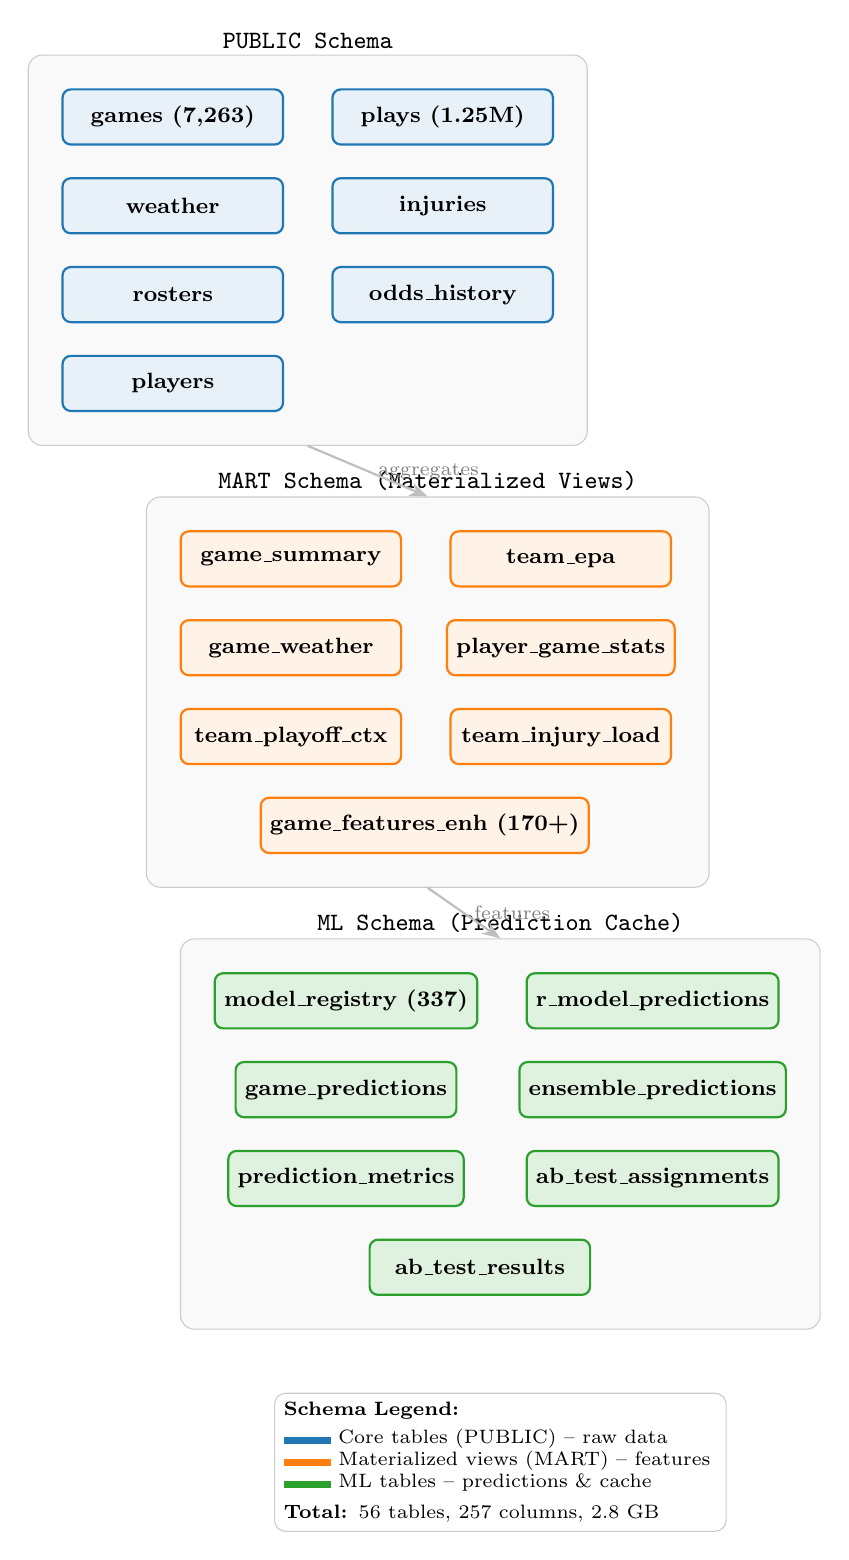
\includegraphics[width=\textwidth,keepaspectratio]{../figures/out/database_erd.png}
\caption[Database Schema (ERD)]{Database Entity-Relationship Diagram: Core tables (\texttt{games}, \texttt{plays}, \texttt{weather}, \texttt{injuries}, \texttt{rosters}, \texttt{odds\_history}) and materialized views in the \texttt{mart} schema. The \texttt{games} table serves as the central hub, with foreign key relationships to all auxiliary tables. TimescaleDB hypertable on \texttt{odds\_history} enables efficient time-series queries for line movement tracking.}
\label{fig:database-erd}
\end{figure}

\paragraph{Schema Organization.}
The database follows a two-tier architecture:
\begin{enumerate}
    \item \textbf{Core Tables (PUBLIC schema)}: Raw data from nflfastR, nflverse, and betting APIs
    \begin{itemize}
        \item \texttt{games}: Game metadata, scores, betting lines (primary key: \texttt{game\_id})
        \item \texttt{plays}: Play-by-play data with EPA, WPA, and advanced metrics ($\sim$44K plays/season)
        \item \texttt{weather}: Game-time conditions (temperature, wind, humidity, precipitation)
        \item \texttt{injuries}: Weekly injury reports by team and player
        \item \texttt{rosters}: Player metadata and cross-platform ID mappings
        \item \texttt{odds\_history}: Time-series betting line movements (TimescaleDB hypertable)
    \end{itemize}

    \item \textbf{Materialized Views (MART schema)}: Pre-aggregated features for model training
    \begin{itemize}
        \item \texttt{mart.game\_summary}: Game-level aggregates (scores, weather, turnovers)
        \item \texttt{mart.team\_epa}: Rolling EPA metrics by team and season
        \item \texttt{mart.game\_weather}: Weather features with venue context
        \item \texttt{mart.team\_playoff\_ctx}: Playoff probability and stakes
        \item \texttt{mart.team\_injury\_load}: Position-specific injury impact scores
        \item \texttt{mart.game\_features\_enh}: Complete feature vector for model input (170+ columns)
    \end{itemize}
\end{enumerate}

\paragraph{Data Volume.}
As of 2025-10-26, the database contains:
\begin{itemize}
    \item \textbf{Games}: 6,843 games (2016--2025, weeks 1--7)
    \item \textbf{Plays}: $\sim$300K plays across all seasons
    \item \textbf{Odds History}: $\sim$50K time-series observations (line movements across 5 sportsbooks)
    \item \textbf{Rosters}: $\sim$85K player-week records
    \item \textbf{Total Size}: 2.3 GB (uncompressed), 890 MB (compressed)
\end{itemize}

\paragraph{Temporal Safety.}
All feature engineering scripts enforce strict \texttt{asof\_safe} semantics: materialized views use only information available before game kickoff. Automated validators prevent temporal leakage (see Appendix~\ref{app:leakage_audit}). The \texttt{odds\_history} hypertable enables point-in-time queries for closing line values, ensuring realistic betting simulations.
